\documentclass[]{article}
\usepackage{lmodern}
\usepackage{amssymb,amsmath}
\usepackage{listings}
\usepackage{graphicx}
\usepackage{subcaption}
\usepackage{hyperref}
\usepackage{bm}

\begin{document}

\section{Information-theoretic Interpretations}
\label{information-theoretic-interpretations}
\indent \indent \textit{by: Isabeau Pr\'emont-Schwarz}
\newline

This post is written for the AIHelsinki study group on natural image
statistics. The content of the post is based on chapter 8 of the Natural Image Statistics book
which is available here \url{http://www.naturalimagestatistics.net/} and the presentation of
this chapter by Vikas Verma, a few derivations have been added. The post is intended as a summary of what was learned
at the AIHelsinki study group on the topic of Information-theoretic interpretations.

We will first talk about the theory before going to some applications. In the theory part we will cover the basic motivation, entropy as a measure of uncertainty, and mutual information. In the applications part we will cover mutual information as used for sparse coding and infomax with nonlinear neurons. 

\subsection{Theory}
\label{theory}
\subsubsection{Motivation}
\label{motivation}
Information theory was first developed in the context of signal transmission. Imagine that we have to transmit messages of the form 

\begin{minipage}{15em}
BABABABADABACAABAACABDAAAAABAAAAAAAADBCA
\end{minipage}

composed of the characters A, B, C, D. With each of the characters having the following probabilities to appear at any given position:

\begin{minipage}{15em}
\centering
$p(A) = 1/2 $
$p(B) =  1/4 $
$p(C) =  1/8 $
$p(D) =  1/8 $
\end{minipage}

Now let's assume we need to code these messages in binary (with 0s and 1s). A naive way of doing this would be to use 2 bits for each letter:

\begin{minipage}{15em}
\centering
$A \rightarrow 00 $
$B \rightarrow 01 $
$C \rightarrow 10 $
$D \rightarrow 11 $
\end{minipage}

This would mean that our 40-letter message would be encoded using 80 bits. But actually we encode our messages more efficiently if instead we use fewer bits for more common letters and more bits for rarer letters. For example, if instead we use one bit for A, 2 bits for B and 3 bits for C and D, for instance:

\begin{minipage}{15em}
\centering
$A \rightarrow 0 $
$B \rightarrow 10 $
$C \rightarrow 110 $
$D \rightarrow 111 $
\end{minipage}

Using this encoding, a typical 40-letter message can be encoded using 
$$ 40 \cdot \big(p(A) \times 1 + p(B) * 2 + p(C) * 3 + p(D) *3\big) = 40 (1/2 + 1/2 +3/8 + 3/8) = 70 bits$$
Thus using this encoding would require 12.5\% fewer bits to send the same message. 
This is actually (as we will see below) the optimal way (using the least amount of bits) of coding our messages in binary. This is what (Shannon) entropy is: \textit{Entropy is the average amount of bits necessary to send a symbol of your message using optimal coding.} Or said another way: \textit{Entropy is the minimum amount of bits necessary (on average) required to send symbols in your message.} 

This means that, denoting the number of bits required to encode $X$ by $l(X)$, we have that the entropy of letter sequences is:
\begin{multline}
\label{eq:predefH}
H = \mathbb{E}(l(X)) = p(A) l(A) + p(B) l(B) + p(C) l(C) + p(D) l(D) = \\
1/2 * 1 + 1/4 * 2 + 1/8 *3 + 1/8 * 3 = 1.75  .
\end{multline}
Thus, on average our letters contain 1.75 bits of information and so its entropy is 1.75.
 
So how do we calculate this Entropy? How do we figure out what is the optimal encoding?

\subsubsection{Entropy as Minimum Coding Length}
\label{entropy-as-minimum-coding-length}

If we define the entropy as the minimum amount of bits required in average for all our symbols, we need to calculate what is the minimum coding length for a given code. 

Finding the minimum coding length, is a simple optimization problem. Assume we have an alphabet of $N$ symbols $X_i$ with $i \in [1,N]$ and symbol $X_i$ has a probability $p(X_i) = p_i$ of appearing at any given position in a message. We further denote $l(X_i) = l_i $ to be the coding length in number of bits for symbol $X_i$. 

What is important to notice at this point is that we can't have 3 different symbols coded with one bit each. We only have 0 and 1. So there is we can have max 2 different symbols coded with one bit. And if we do have two symbols coded with a single bit, say $A\rightarrow 0$ and $B\rightarrow 1$, then we cannot represent any other symbol because A and B already occupy the whole coding space, 0001110 already means AAABBBA. So a symbol coded with 1 bit takes up $1/2$ of the coding space. And in general a symbol coded with $l$ bits takes up $2^{-l}$ of the coding space. So we are constrained by 
\begin{equation}
\label{ineq:coding-constraint}
\sum_{i = 0}^N 2^{-l_i} \leq 1 .
\end{equation}
 But to be optimal we wish to use the whole coding space so we want to satisfy the constraint
 \begin{equation}
\label{eq:coding-constraint}
\sum_{i = 0}^N 2^{-l_i} = 1 .
\end{equation}

So out goal is to minimize 
\begin{equation}
\label{eq:objfct}
\mathbb{E}(l_i) = \sum_{i=0}^N p_i l_i ,
\end{equation}
under constraint (\ref{eq:coding-constraint}).  And so using a Lagrange multiplier $\lambda$ to enforce the constraint we need to extremize:
\begin{equation}
\label{eq:exfct}
\sum_{i=0}^N p_i l_i  + \lambda \big(\sum_{i = 0}^N 2^{-l_i} -1\big) .
\end{equation}

Which means we get differentiating with respect to $l_i$:
\begin{equation}
\label{eq:expresols}
p_i   - \lambda \ln(2) 2^{-l_i} = 0 .
\end{equation}

And so solving for $l_i$ we get
\begin{equation}
\label{eq:mincodinglen}
l_i = -\log_2(p_i) .
\end{equation}

This means that for optimal minimal length coding, a symbol $X$ should be coded using $\log_2(p(X))$ bits. We can now check that our second coding in the above section was optimal. We indeed had:
\begin{align}
\label{ex:optcode}
l(A) = & 1 = - \log_2(1/2) = \log_2(p(A)) \\
l(B) = &  2 = - \log_2(1/4) = \log_2(p(B)) \\
l(C) = & 3 = - \log_2(1/8) = \log_2(p(C)) \\
l(A) = & 3 = - \log_2(1/8) = \log_2(p(D)) .
\end{align}

We can plugin our new-found result (\ref{eq:mincodinglen}) in (\ref{eq:predefH}) to obtain:

\begin{multline}
\label{eq:defH}
H = \sum_{i=0}^N p_i l_i = -\sum_{i=0}^N p_i \log_2(p_i) .
\end{multline}

And this is how we will actually define the entropy. Notice that in sum case, it might be impossible to realize the minimal coding length in practice because it would require a fractional number of bits for some symbols. But even in those case we will define the entropy to be (\ref{eq:defH}) even if the minimal coding length cannot be achieved in practice. With this definition we have that the entropy is the expected number of bits of information which we will acquire for every new symbol we receive. 

\subsubsection{Differential Entropy}
\label{differential-entropy}

So far we have talked about discrete random variables, for which we defined the entropy to be
\begin{equation}
\label{eq:defH2}
H =  -\sum_{i=0}^N p_i \log_2(p_i) ,
\end{equation}
for an entropy calculated in units of bits or 
\begin{equation}
\label{eq:defHnat}
H =  -\sum_{i=0}^N p_i \log_e(p_i) = -\sum_{i=0}^N p_i \ln(p_i) ,
\end{equation}
for an entropy calculated in units of nats (natural unit of information). Note that since the probabilities $p_i$ are always between 0 and 1, $-\log(p_i)$ is always positive and so entropy is always positive, this will not always be the case in the continuous case. But how should we define entropy in the continuous random variable case? Well, like one normally does in those cases, we simply replace the sum by an integral:
\begin{equation}
\label{eq:defHcont}
H =  -\int_{x=-\infty}^{+\infty} p(x) \log(p(x)) dx ,
\end{equation}
where $p(x)$ is now the probability density function. 

Back in the discrete case, entropy was somewhat intuitively understood as the number of bits on carried on average by one reading of the value of the random variable and intuition was a good guide as to what to expect. Intuition is not a very good guide anymore in the continuous case. To see this, let us consider the case of the uniform distribution on the interval $[0,\alpha]$:
\begin{align}
\label{uniformdist}
  p(x) = \begin{cases}
    \frac{1}{\alpha}, & \text{if $0 \leq x \leq \alpha$}\\
    0, & \text{otherwise.}
\end{cases}
\end{align}
Which gives us an entropy of: 
\begin{equation}
\label{eq:uniH}
H(x) =  -\int_{x=0}^{+\alpha} \frac{1}{\alpha} \log(\frac{1}{\alpha}) dx  = \log(\alpha) .
\end{equation}

From this we see that depending on the value of $\alpha$, the entropy can be negative ($\alpha < 1$, zero $\alpha = 1$, or positive $\alpha > 1$, and it ranges from $-\infty$ ($\alpha \rightarrow 0^+$) to $+\infty$ ($\alpha \rightarrow +\infty$).  Conceptually the entropy of a continuous variable can be negative because, compared to the discrete case, we omit an infinite component.  We can compare the differential entropy to the discrete entropy by discretizing the continuous variable and calculating the discrete entropy for it. Let us consider a continuous random variable which takes values in the interval [0,1] with probability density function $p(x)$ with $p(x) = 0$ for $x>1$ or $x<0$. We transform it into a discrete probability problem by dividing the interval [0,1] into $n$ bins of size $1/n$. Bin $i$ is the interval $[\frac{i-1}{n}, \frac{i}{n}]$. We thus have that the probability $p_i$ that variable falls in bin $i$ is 
\begin{equation}
\label{eq:pi}
p_i =  -\int_{x=\frac{i-1}{n}}^{+\frac{i}{n}} p(x)  dx  \approx p(\frac{i}{n})\cdot\frac{1}{n} ,
\end{equation}
where the approximation is valid for a continuous $p(x)$ when the intervals are small enough ($n$ large enough).  Therefore the entropy for the discrete process of ending up in different bins is 
\begin{align}
\label{eq:Hrel}
H_{discrete} & =  -\sum_{i=0}^N p_i \log(p_i)  \approx -\sum_{i=0}^N p(\frac{i}{n}) \log(\frac{p(\frac{i}{n})}{n})\cdot \frac{i}{n} \\
& =  -\sum_{i=0}^N p(\frac{i}{n}) (\log(p(\frac{i}{n})) -\log(n)) \cdot \frac{i}{n}  \\
& \approx -\int_{x=0}^1 p(x) (\log(p(x)) -\log(n)) dx \\
& = H_{differential} + \log(n) . 
\end{align}

As the continuous case is obtained from the discrete case by taking the limit $n\rightarrow \infty$, we see that differential entropy is equal to the discrete entropy minus a constant infinite component (equal to $\log(\aleph_0) = \aleph_0$) which is the same for all continuous distributions. As such, differential entropy should be thought of not as absolute but as relative to other entropy values. 

A natural question to ask at this point is what distribution has the maximum entropy. Of the distributions with support on the interval [0,1], the uniform distribution is that with maximal entropy as one would intuitively expect: we gain the most information by reading the value of the random variable if all values were equally likely.  But, of the distributions on $[-\infty, +\infty]$ with unit variance, what is the distribution with maximum entropy? That is a less trivial question. We can answer that question using calculus of variations. Further constraining the mean to be 0 (the problem is translation invariant), we wish to maximize 
\begin{equation}
\label{eq:maxentfct}
H =  -\int_{x=-\infty}^{+\infty} p(x) \big(\log(p(x)) +\lambda(x^2-1) +\mu + \rho (x-0)\big) dx  +\mu,
\end{equation}
where the second term with the Lagrange multiplier $\lambda$ is to impose the unit variance constraint, the Lagrange multiplier $\mu$ is to impose the constraint that the integral of $p(x)$ should be one, and the Lagrange multiplier $\rho$ is to impose zero mean. Using calculus of variations we have 
\begin{equation}
\label{eq:dmaxentfct}
\delta H =  -\int_{x=-\infty}^{+\infty} \delta p(x) \big(\log(p(x)) +\lambda(x^2-1) +1 +\mu + \rho x\big)  dx .
\end{equation}

Thus our distribution must satisfy
\begin{align}
\label{eq:maxentsol}
\log(p(x)) +\lambda(x^2-1) +1 +\mu +\rho x = 0 \\
p(x) = \exp\big(-\lambda(x^2-1) -1 -\mu -\rho x\big).
\end{align}
Solving for $\lambda$, $\mu$, and $\rho$ using the constraints we finally have that
\begin{equation}
\label{eq:maxentsol2}
p(x) = \frac{1}{\sqrt{2\pi}}e^{-x^2/2} ,
\end{equation}
which is the normal distribution with mean zero and unit variance. We thus conclude that for a given fixed variance, the distribution with the maximum entropy is the Gaussian distribution. Thus in some sense, the Gaussian distribution is the "most random" distribution, the "least deterministic" one. Viewed in the way, the central limit theorem, which says that the average of independent identically distributed variables tends towards the Gaussian in the infinite limit, is not so surprising: adding randomness by adding more independent variables will converge to the most random of all distribution, the Gaussian distribution. 

\subsubsection{Mutual Information}
\label{mutual-information}

Suppose you have two random variables $x$ and $y$ and that $x$ and $y$ might not be independent. The probability of $x$ given $y$, $p(x|y)$, is the conditional probability of $x$ given $y$. The entropy for this conditional probability distribution is 
\begin{equation}
\label{eq:condHk}
H =  -\sum_{i=0}^N p(x_i|y_k) \log(p(x_i|y_k)) ,
\end{equation}
for some $k$. If we average this entropy over all possible values of $y$, we get what is called the \textit{conditional entropy}:
\begin{equation}
\label{eq:condH}
H(x|y) =  -\sum_{k=0}^M\sum_{i=0}^N p(y_k) p(x_i|y_k) \log(p(x_i|y_k)) ,
\end{equation}
which tells us on average how much more (bits of) information we get on average by knowing the value of $x$ if we already know the value $y$. Notice that if $x$ and $y$ are independent so that $p(x|y) = p(x)$ then we have that $H(x|y) = H(x)$. 

In the above we wrote down the equations for discrete random variables, but exactly the same considerations apply for continuous variable simply by replacing the sum with an integral. In this section, unless explicitly mentioned everything we derive or say will apply equally well to the discrete and continuous case (simply by switching between sums and integrals) unless we say so explicitly. 

Knowing that $p(x|y) = \frac{p(x,y)}{p(y)}$ we have that
\begin{align}
\label{id:condH}
H(x|y) & =  -\sum_{k=0}^M\sum_{i=0}^N p(y_k) p(x_i|y_k) \log(p(x_i|y_k)) \\
& = -\sum_{k=0}^M\sum_{i=0}^N p(y_k) \frac{p(x_i,y_k)}{p(y_k)} \log(\frac{p(x_i,y_k)}{p(y_k)}) \\
\label{interHcond}
&  = -\sum_{k=0}^M\sum_{i=0}^N p(x_i,y_k)\log(p(x_i,y_k)) + \sum_{k=0}^M\sum_{i=0}^N p(x_i,y_k)\log(p(y_k)) \\
& = H(x,y) - H(y) ,
\end{align}
where $H(x,y)$ is the entropy of the combined variables $x$ and $y$. 

Mutual information, $I(x,y)$, between $x$ and $y$, is the information which is shared by $x$ and $y$, so it is the information contained in $x$ ($H(x)$) minus the information in $x$ which is not in $y$ ($H(x|y)$):
\begin{align}
\label{eq:MI}
I(x,y) & =  H(x) - H(x|y) \\
& = H(x) + H(y) -H(x,y) \\
\label{gibbsformat}
& =  \Big( -\sum_{k=0}^M\sum_{i=0}^N p(x_i,y_k)\log(p(x_i)p(y_k))\Big)-\Big( -\sum_{k=0}^M\sum_{i=0}^N p(x_i,y_k)\log(p(x_i,y_k))\Big) \\
\label{MIcondensed}
&  = -\sum_{k=0}^M\sum_{i=0}^N p(x_i,y_k)\log\big(\frac{p(x_i) p(y_k)}{p(x_i,y_k)}\big) ,
\end{align}
where $p(x_i) = \sum_{k=0}^M p(x_i,y_k)$ is the marginal distribution of $x$ and $p(y_k) = \sum_{i=0}^N p(x_i,y_k)$ is the marginal distribution of $y$. 
\begin{figure}
      \centering
      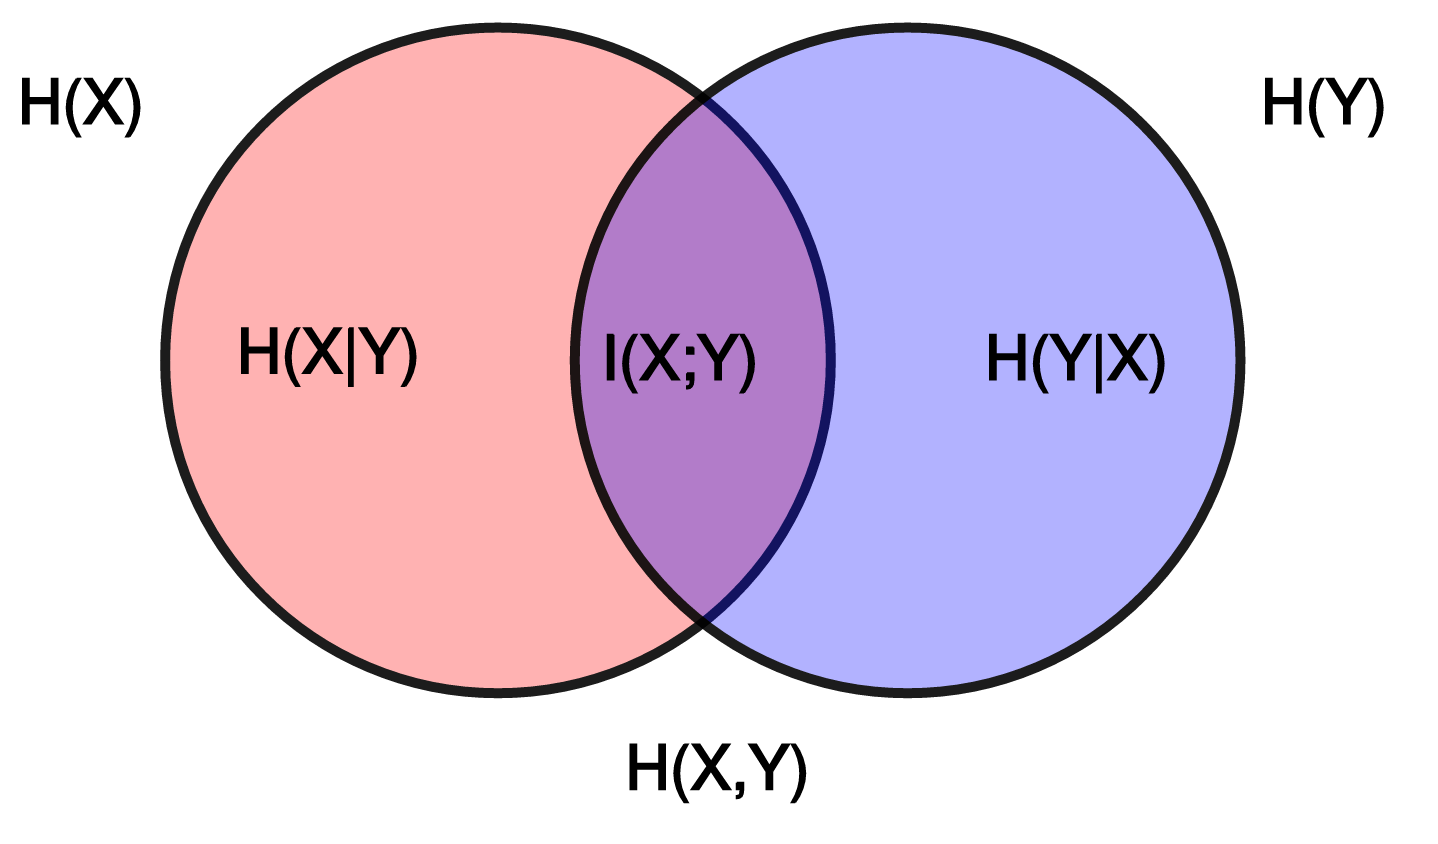
\includegraphics[width=1.\linewidth]{entropyvenn.png}
    \caption{The area contained by both circles is the joint entropy $H(X,Y)$. The circle on the left (red and violet) is the individual entropy $H(X)$, with the red being the conditional entropy $H(X|Y)$. The circle on the right (blue and violet) is $H(Y)$, with the blue being $H(Y|X)$. The violet is the mutual information $I(X;Y)$. Image source: Wikipedia.}
    \label{fig:venn}
\end{figure}

At this point it is useful to look at Gibbs' inequality which states that for two probability distributions $r$ and $q$
\begin{equation}
\label{Gibbs}
- \sum_{i=0}^N r_i \log(r_i) \leq - \sum_{i=0}^N r_i \log(q_i) ,
\end{equation}
or in the continuous case that
\begin{equation}
\label{Gibbs}
- \int r(x) \log(r(x)) dx \leq - \int r(x) \log(q(x)) ,
\end{equation}
with equality if and only if $r = q $. By applying Gibbs' inequality to (\ref{gibbsformat}), with $r = p(x,y)$ and $q = p(x)p(y)$, we see that the mutual information $I(x,y)$ is always positive and is equal to zero if and only if $p(x,y) = p(x)p(y)$. In other words, this means that the mutual information is non-negative and it is zero if and only if $x$ and $y$ are independent variables. Looking at (\ref{eq:MI}) this also means that 
\begin{equation}
\label{Hcondsmaller}
  H(x) \geq H(x|y) ,
\end{equation}
with equality if and only if $x$ and $y$ are independent random variables.


So in conclusion, we see that $H(x,y)$, $H(x)$, $H(x|y)$, and $I(x,y)$ fit together like in the Venn diagram of Fig. \ref{fig:venn}. But remember that while for discrete variables, all of these components are non-negative, this is not true for the continuous case where  $H(x)$, $H(x|y)$, and $H(x,y)$ can all be negative, only $I(x,y)$ is always non-negative even in the continuous case. 

\subsection{Applications}
\label{applications}
\subsubsection{Sparse Coding}
\label{sparse-coding}

Now that we have developed this these information-theoretic tools, we can look at sparse coding and ICA from an information-theoretic perspective. In sparse coding and ICA we have signals $z_i$ (which are usually whitened) and we want to find sparse sources $s_j$ for these signals by orthogonally rotating the $z$'s:
\begin{equation}
\label{sparsetransformation}
s_j = \sum_i v_{j i} z_i .
\end{equation}

We denote $H(\bm{z}) = H(z_1,\ldots, z_N)$ and $\bm{s} = \bm{v \cdot z}$.  If $\bm{v}$ is an orthonormal matrix, we are only rotating the probability space so that 
\begin{align}
\label{sameent}
H(s_1, \ldots, s_N) & = H(\bm{s}) \\
& = H((\bm{v\cdot z})_1, \ldots, (\bm{v\cdot z})_N) \\
& = H(\bm{v\cdot z}) \\
& = H(\bm{z}) \\
& = H(z_1,\ldots, z_N) .
\end{align}

So in ICA or in spare coding, if the sparsity function is $h(s^2) = \log(p(s))$, we try to minimize
\begin{equation}
\label{icaopt}
\sum_i H(s_i) = \sum_i H((\bm{v\cdot z})_i) .
\end{equation}
But in the case in which $\bm{v}$ is orthonormal, that is the same as minimizing
\begin{align}
\label{caopt2}
\left(\sum_i H(s_i)\right) - H(\bm{z}) &  = \left(\sum_i H(s_i)\right) - H(\bm{v\cdot z}) \\
& = \left(\sum_i H(s_i)\right) - H(\bm{s}). 
\end{align}
And from the definition of mutual information (equation (\ref{eq:MI})) we have that
\begin{align}
\label{icaopt3}
\left(\sum_i H(s_i)\right) - H(\bm{s}) = \sum_{K=2}^N \sum_{\{i_1,\ldots,i_K \}\in \{1,\ldots,N\}} (K-1) \cdot I(x_{i_1},\ldots,x_{i_K}|x_j \text{s.t.} j\notin\{i_1,\ldots,i_K \}), 
\end{align}
so we see that in this case, both ICA and sparse coding are equivalent to minimizing the mutual information between the sources to have the sources be as independent as possible. 


\subsubsection{Infomax with Nonlinear Neurons}
\label{infomax}

Let us consider a neuron-network layer which has (nonlinear) activation function $\phi$ and input vector $\bm{x}$ which is considered to be continous-valued. Let $\bm{b}$ be a transformation matrix on $\bm{x}$. Then we have that the activation of neuron $i$ is
\begin{equation}
\label{neuronact}
y_i = \phi((\bm{b \cdot x})_i) +n_i,
\end{equation}
where $n$ is some independent (Gaussian) noise. 

The principle behind infomax is to try to keep as much information about $\bm{x}$ in $\bm{y}$. Thus we want to maximize the mutual information between $\bm{x}$ and $\bm{y}$
\begin{equation}
\label{infomaxmax}
 I(\bm{x},\bm{y}) = H(\bm{y}) -H(\bm{y}|\bm{x}).
 \end{equation}
 But because $p(\bm{y}|\bm{x}) = p(\bm{n})$ doesn't depend on $\bm{b}$ we can forget about the $H(\bm{y}|\bm{x})$ and just try to maximize the entropy of $\bm{y}$, $H(\bm{y})$.
 
 \begin{align}
\label{deriveinfomax}
H(\bm{y}) & = -\int p_y(\bm{y}) \log(p_y(\bm{y})) d\bm{y} \\
& = -\int p_x( \bm{x} ) \log(p_y( \phi(\bm{b \cdot x}))) d\bm{x} \\
& = -\int p_x( \bm{x} )\left(\log(p_x(\bm{x})) - (\sum_{i=0}^N \log(\phi^\prime((\bm{b \cdot x})_i))) - \log(\det(\bm{b}))\right)\\
& = H(\bm{x}) + \sum_i \mathbb{E}_x\left(\log(\phi^\prime((\bm{b \cdot x})_i))\right) + \log(\det(\bm{b})) .
\end{align}
Where we used the fact that  
 \begin{align}
\label{probident}
p_y( \bm{y}) d\bm{y} & = p_x(\bm{x})  d\bm{x} \\
p_y( \bm{y}) & = p_x(\bm{x}) (\det(\frac{d\bm{y}}{d\bm{x}} ))^{-1} \\
& = p_x(\bm{x}) \cdot \left(\prod_{i=0}^N \phi^\prime((\bm{b \cdot x})_i) \cdot \det(\bm{b})\right)^{-1}.
\end{align}

Because $ H(\bm{x}) $ does not depend on $\bm{b}$, we can drop it and simply maximize
\begin{equation}
\label{finalinfomax}
\sum_i \mathbb{E}_x\left(\log(\phi^\prime((\bm{b \cdot x})_i))\right) + \log(\det(\bm{b})) .
\end{equation}
At this point, we may notice that that is this equation has the same form as the one which one must maximize in the ICA model where the probability density functions are replaced by the derivatives of the activation function $\phi^\prime$. This means that if one choses the cumulative distribution functions of the densities $p_i$'s of the Independent Components as the activation functions $phi$, then we have that infomax is equivalent to the maximum likelihood estimation of the ICA model.  In particular, using the sigmoid activation function 
\begin{equation}
\label{sigmoid}
\phi(x) = \frac{1}{1+e^{-x}} ,
\end{equation}
then $\phi^\prime$ is a sparse distribution, and in fact $\log(\phi^\prime)$ is the commonly used measure of sparsity, the log-cosh function. This ties together ICA, sparse coding, and infomax.  
\end{document}